\documentclass[10pt,a4paper]{article}
\usepackage[utf8]{inputenc}
\usepackage[spanish]{babel}
\usepackage{amsmath}
\usepackage{amsfonts}
\usepackage{amssymb}
\usepackage{enumitem}
\usepackage{hyperref} 
\usepackage{graphicx}
\hypersetup{pdftex,colorlinks=true,allcolors=blue}
\hypersetup{
    pdftitle={},
    pdfauthor={Pablo Riutort Grande},
    pdfsubject={},
    bookmarksnumbered=true,     
    bookmarksopen=true,         
    bookmarksopenlevel=1,       
    colorlinks=true,            
    pdfstartview=Fit,           
    pdfpagemode=UseOutlines,    % this is the option you were lookin for
    pdfpagelayout=TwoPageRight
}
\usepackage{listings}
\usepackage{xcolor}
\usepackage{hypcap}
\definecolor{codegreen}{rgb}{0,0.6,0}
\definecolor{codegray}{rgb}{0.5,0.5,0.5}
\definecolor{codepurple}{rgb}{0.58,0,0.82}
\definecolor{backcolour}{rgb}{0.95,0.95,0.92}
\lstdefinestyle{mystyle}{
    backgroundcolor=\color{backcolour},   
    commentstyle=\color{codegreen},
    keywordstyle=\color{magenta},
    numberstyle=\tiny\color{codegray},
    stringstyle=\color{codepurple},
    basicstyle=\ttfamily\footnotesize,
    breakatwhitespace=false,         
    breaklines=true,                 
    captionpos=b,                    
    keepspaces=true,                 
    numbers=left,                    
    numbersep=5pt,                  
    showspaces=false,                
    showstringspaces=false,
    showtabs=false,                  
    tabsize=2
}
\lstset{style=mystyle}
\usepackage{xparse}
\NewDocumentCommand{\codeword}{v}{%
\texttt{{#1}}
}
\author{Pablo Riutort Grande}
\title{Identidad Digital\\ \vspace{1cm}\textbf{Segunda Práctica (PRAC2)}}
\begin{document}
\maketitle
\pagebreak

\section*{Introducción}
Este documento recoge los pasos a seguir para la resolución de la segunda práctica de la asignatura de Identidad Digital. Se compone de dos apartados: Preparación y Desarrollo donde se explican los pasos a seguir para preparar el entorno sobre el cuál se ha ejecutado la práctica, la creación y modificación del software necesario para asumir los objectivos de seguridad propuestos por la práctica y, finalmente, se explica cómo estos factores culminan el la aplicación IDwebapp y el servidor CAS que cumple con los requisitos de la práctica en forma de aplicación web.

\section*{Preparación}
El entorno de la práctica se compone de los siguientes elementos:
\begin{itemize}
\item Java SE Development Kit (JDK) v9.0.4.11+
\item Apache Tomcat 9.0.27
\end{itemize}

A continuación se espeficica un listado de archivos que fueron modificados para la correcta ejecución de la práctica, todos estos archivos se adjuntan en la entrega del ejercicio:\\

\textbf{manage.sh}: script auxiliar para gestionar la aplicación.\\

\textbf{APP}
\begin{itemize}
\item web.xml en \codeword{webapps/IDwebapp/WEB-INF/web.xml}
\item applicationContextSecurity.xml en \\ \codeword{webapps/IDwebapp/WEB-INF/applicationContextSecurity.xml}
\item menu.jsp situado en \codeword{webapps/IDwebapp/secure/menu.jsp}
\item index.jsp situado en \codeword{webapps/IDwebapp/index.jsp}
\item server.xml situado en \codeword{conf/server.xml}
\end{itemize}
\vspace{.3cm}

\textbf{CAS}
\begin{itemize}
\item pom.xml situado en \\ \codeword{webapps/cas-server-webapp-4.0.0/META-INF/maven/.../pom.xml}
\item deployerConfigContext.xml situado en \\ \codeword{webapps/cas-server-webapp-4.0.0/WEB-INF/deployerConfigContext.xml}
\item cas.properties situado en \codeword{cas-server/WEB-INF/cas.properties}
\item server.xml situado en \codeword{conf/server.xml}
\end{itemize}

\subsection*{URLs de la aplicación}
La URL de acceso a la aplicación APP es \codeword{localhost:8080/IDwebapp} y el servidor CAS se encuentra escuchando en \codeword{localhost:8090/cas-server-webapp-4.0.0/}

\section*{Desarrollo}
Recordemos que el desarrollo de este proyecto consiste en replicar la arquitectura (Fig. \ref{fig:arch}).
\begin{figure}[h!]
  \centering
   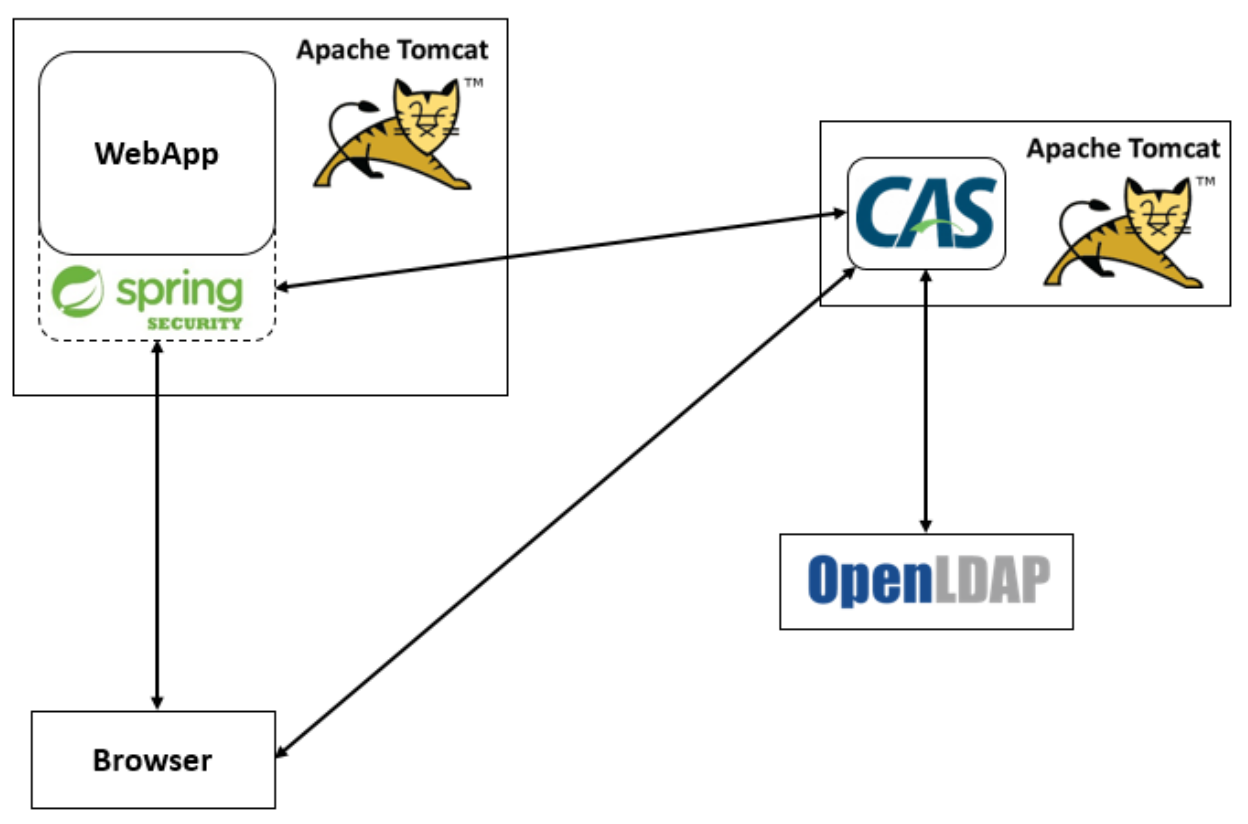
\includegraphics[scale=0.2]{architecture.png}\\
  \caption{APP utiliza el framework Spring security para validarse contra el CAS que obtiene los datos del servidor LDAP}
  \label{fig:arch}
\end{figure}\\

A continuación se especifica en detalle qué cambios fueron efectuados en los archivos listados en el apartado anterior para cumplir con los requisitos de la práctica.

\subsection*{manage.sh}
Se ha añadido el siguiente script que levanta y detiene ambas aplicaciones con los comandos \codeword{run} y \codeword{stop} respectivamente.
\lstinputlisting[language=bash]{manage.sh}


\subsection*{APP}
APP es el antiguo IDwebapp que ha sido reconfigurado para utilizar un CAS (\textit{Central Authentication Service}) a través de Spring security framework.

\subsubsection*{web.xml}
En esta iteración de la aplicación el archivo web contiene referencias al framework de Spring security para gestionar el acceso de usuarios. Recordemos que anteriormente era este archivo quien gestionaba la lógica de acceso y definición de roles.\\
Hay que destacar la referencia al archivo \codeword{applicationContext-security.xml}, donde pasan a definirse las restricciones:
\lstinputlisting[language=XML,firstline=13,lastline=18]{appweb.xml}

Y también las referencias al Spring security framework:
\lstinputlisting[language=XML,firstline=25,lastline=48]{appweb.xml}

\subsubsection*{applicationContext-security.xml}
Este archivo se añade para gestionar el cotrol de acceso a los recursos con Srping así como para también definir los roles de los usuarios. Este archivo viene a sustituir el anterior web.xml de la misma aplicación.\\

Se definen las secciones y a qué tiene acceso cada rol.
\lstinputlisting[language=XML,firstline=20,lastline=34]{applicationContext-security.xml}
\vspace{.3cm}


Se configura la aplicación para conectarse al servidor CAS para la autenticación. Definimos el CAS como \codeword{authenticationProvider} según Spring\\
\lstinputlisting[language=XML,firstline=37,lastline=83]{applicationContext-security.xml}

Finalmente, también se definen los roles de cada usuario:
\lstinputlisting[language=XML,firstline=85,lastline=95]{applicationContext-security.xml}


\subsubsection*{menu.jsp}
En el archivo \codeword{menu.jsp} ahora se revisa la pertenencia del usuario a los distintos roles con una comprobación manual similar a la de enseñar a qué secciones puede acceder cada rol en la aplicación:
\lstinputlisting[language=HTML,firstline=12,lastline=31]{menu.jsp}

De esta forma se consigue ver a qué roles pertenece el usuario a modo de lista junto a su nombre.\\

También hay que destacar que ahora el logout de la aplicación lo hace el \codeword{j_spring_security_logout}:
\lstinputlisting[language=HTML,firstline=108,lastline=108]{menu.jsp}


\subsubsection*{index.jsp}
En archivo \codeword{index.jsp} antes gestionaba el logout del request. Ahora solo es necesario definir las siguientes cabeceras para delegar en Spring security:
\lstinputlisting[language=HTML,firstline=1,lastline=4]{index.jsp}

\subsubsection*{server.xml}
Este archivo deja de tener el Realm que define \codeword{userClassNames} y \codeword{roleClassNames} ahora gestionado por Spring.

\subsection*{CAS}
En esta práctica tenemos que gestionar el control de acceso de los usuarios de APP a través de un CAS que se conectar a un servidor LDAP cuyo contenido está previamente definido en el ejercicio 1. \\

A continuación se define la configuración de este proyecto Tomcat para su correcto funcionamiento.

\subsubsection*{pom.xml}
Maven es un gestor de dependencias para instalar paquetes externos dentro de una aplicación. Los paquetes necesarios para la aplicación que gestiona Maven se describen en el fichero pom.xml. En nuestro caso, añadimos al pom suministrado la dependencia de LDAP:
\lstinputlisting[language=XML,firstline=57,lastline=61]{pom.xml}

\subsubsection*{web.xml}
De igual forma que en la APP se define el contexto de la aplicación en cuanto a gestión de autenticación, en el CAS se definen los parámetros que deben ser considerados para su correcto funcionamiento, en concreto se especifica el archivo deployerConfigContext que es de suma relevancia en esta prática:
\lstinputlisting[language=XML,firstline=28,lastline=34]{casweb.xml}

\subsubsection*{deployerConfigContext.xml}
Este archivo es el que configura la conexión al servidor LDAP. En él se definen los distintos aspectos necesarios para esta conexión a través de dinstintos beans.\\

Cabe destacar que la estrategia elegida para la conexión con LDAP es el \textit{direct bind}. Este modo de conexión se puede realizar si:
\begin{enumerate}
\item Todos los usuarios cuelgan de una misma rama en el directorio. En nuestro caso será \textit{employees}.
\item El \textit{username} que se le da al CAS forma parte del \textit{dn}. En nuestro caso se define precisamente así:\\
 \codeword{dn: uid=<username>,ou=employees,dc=insectores,dc=com}
\end{enumerate}

Algunos beans a destacar:
\begin{itemize}
\item \codeword{authenticationManager}. En este bean se definen los gestores de autenticación. Deberemos añadir el del LDAP.
\lstinputlisting[language=XML,firstline=54,lastline=69]{deployerConfigContext.xml}
\item \codeword{ldapAuthenticationHandler}. Definimos cómo se mapean los atributos del servidor LDAP a nuestra aplicación.
\lstinputlisting[language=XML,firstline=126,lastline=144]{deployerConfigContext.xml}
En concreto en \codeword{<entry key="cn" value="cn" />}
\item \codeword{dnResolver}. 
\lstinputlisting[language=XML,firstline=154,lastline=156]{deployerConfigContext.xml}
\item \codeword{connectionConfig}. Define cómo hay que conectarse al servidor LDAP.
\lstinputlisting[language=XML,firstline=184,lastline=188]{deployerConfigContext.xml}
\item \codeword{sslConfig}
\lstinputlisting[language=XML,firstline=190,lastline=195]{deployerConfigContext.xml}
\end{itemize}

Todos los parámetros vendrán dados por el fichero cas.properties. De esta forma podemos hacer un control más modular de la aplicación.

\subsubsection*{cas.properties}
En este fihcero de properties podemos definir los parámetros necesarios para la conexión del CAS con LDAP de manera cómoda y modular.\\

Podemos destacar que aquí es donde se define la dirección del servidor LDAP:
\lstinputlisting[firstline=48,lastline=58]{cas.properties}

Esta URL tiene que ser la misma que la del servidor LDAP de localhost (Fig. \ref{fig:ldap}).
\begin{figure}[h!]
  \centering
   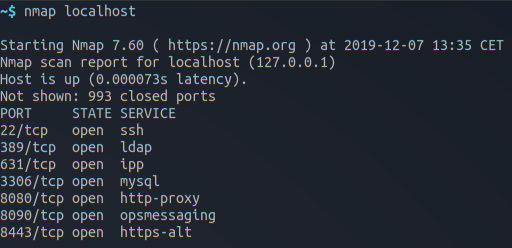
\includegraphics[scale=0.6]{nmap.png}\\
  \caption{La dirección de LDAP es \textit{localhost:389}}
  \label{fig:ldap}
\end{figure}\\
\pagebreak

También se define la autenticación en LDAP: qué nodo contiene los usuarios a autenticar, el password para acceder al servidor desde CAS y definición de los filtros de búsqueda
\lstinputlisting[firstline=83,lastline=101]{cas.properties}

Podemos destacar que también se pueden definir opciones para securizar la aplicación, tratadas en el último requisito de la práctica:
\lstinputlisting[firstline=103,lastline=103]{cas.properties}

Todas estas configuraciones son necesarias para el deployerConfigContext para que pueda hacer una búsqueda satisfactoria de usuarios en LDAP.

\subsubsection*{server.xml}
Para evitar colisiones entre los dos proyectos de Tomcat, se ha optado por cambiar el puerto de escucha de la aplicación CAS, en conreto esta aplicación escuchará al puerto 8090.\\
\lstinputlisting[firstline=69,lastline=71]{server.xml}

\section*{Apéndice}
\subsection*{Utilización SSL (y certificados) para proteger las comunicaciones}
Lamentablemente este punto no se ha podido tratar satisfactoriamente en esta entrega. Como nota personal, el uso de Tomcat me ha resultado difícil y tedioso por lo que completar este punto ha sido frustrado por la poca familiaridad que tengo con este framework, lo difícil que me ha resultado aplicar la documentación tanto suministrada como encontrada por internet y por la falta de tiempo a estas alturas de la práctica.

\end{document}